%% ====================================================================
%%  Chapter 5 — Results and Discussion
%% ====================================================================
\chapter{Results and Discussion}
\label{ch:results}

The results of the proposed model evaluations are presented in this chapter, along with a discussion of
each result.

\section{In-Distribution Accuracy}
\label{sec:res:indist}

Table~\ref{tab:res:baseline} presents the accuracy of each student model on the test set of Session 2,
and Figure~\ref{fig:res:cdf_indist} presents the distribution of per-sample error for each of the three
convolutional student models.

\begin{table}[H]
\centering
\caption{In-distribution localization accuracy (Session~2 test set, $N = 4{,}260$). Student models
trained for 50 epochs; U-Net variants for 120 epochs. \best{Green bold} = best in column.}
\label{tab:res:baseline}
\begin{tabular}{@{}lrcccc@{}}
\toprule
\textbf{Model} & \textbf{Params} & \textbf{Mode} & \textbf{Median (m)} & \textbf{P90 (m)} & \textbf{P99 (m)} \\
\midrule
DLoc baseline    & 16.5M & ---        & 0.707 & $\sim$1.6 & $\sim$4.0 \\
\midrule
MobileNetV2      & 2.3M  & Standalone & 0.707 & 1.616 & 3.992 \\
MobileNetV2      & 2.3M  & Distilled  & 0.707 & 1.612 & 4.003 \\
\midrule
TinyCNN          & 47K   & Standalone & 3.922 & 13.919 & 23.244 \\
TinyCNN          & 47K   & Distilled  & 3.706 & 14.784 & 25.101 \\
\midrule
Mamba            & 0.65M & Standalone & 10.56 & 20.0 & 28.3 \\
\midrule
MobileNetV2-UNet & 2.41M & Standalone (Cosine) & \best{0.640} & 1.523 & 2.750 \\
MobileNetV2-UNet & 2.41M & Standalone (Step)   & \best{0.640} & 1.552 & 2.918 \\
MobileNetV2-UNet & 2.41M & Distilled (Cosine)  & \best{0.640} & \best{1.513} & \best{2.587} \\
\bottomrule
\end{tabular}
\end{table}

\begin{figure}[H]
\centering
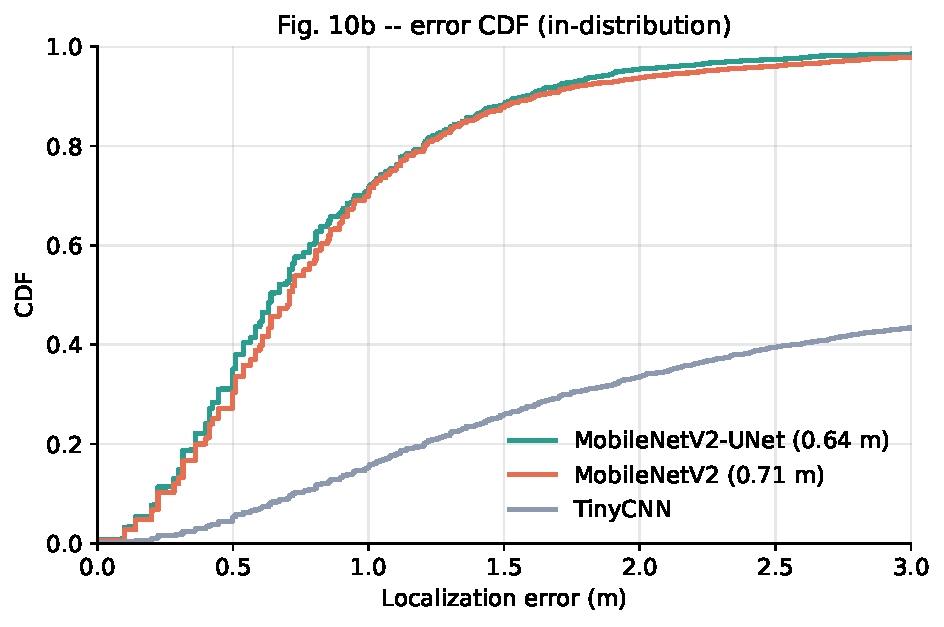
\includegraphics[width=0.78\linewidth]{cdf_fig10b.pdf}
\caption{Cumulative distribution of in-distribution localization error. The MobileNetV2-UNet
(0.64\,m median) lies above the plain MobileNetV2 (0.71\,m) across the full range, while TinyCNN trails
far behind, never reaching the 0.8 CDF level within 3\,m.}
\label{fig:res:cdf_indist}
\end{figure}

The MobileNetV2 model achieves a lossless $7.2\times$ compression of the DLoc baseline model. The
MobileNetV2 model achieves the same 0.707\,m median error as the DLoc model, indicating that it can
achieve the same accuracy with fewer parameters. This indicates that the DLoc model is over-parameterized
for in-distribution modeling: a model with 2.3~million parameters is able to achieve the same accuracy as
a model with 16.5~million parameters.

The TinyCNN model is limited by its model capacity. The TinyCNN model reaches a median error of
3.922\,m, five times the error of the baseline model. TinyCNN has only three convolutional layers, and it
is likely that the model is too small to effectively learn both the per-AP features and the spatial
features of the location. The P90 of the TinyCNN model (the point at which 90\% of predictions are within
the given distance of the true location) is 13.9\,m. Approximately 2~million parameters are required for
this task; with fewer parameters than this floor, no amount of training achieves the accuracy required to
localize objects in these images.

The Mamba model fails to learn the localization task. With 0.65~million parameters, it reaches a median
error of only 10.56\,m---the worst of any model evaluated, and the reason it sits at the top of the
accuracy--size plane in Figure~\ref{fig:res:pareto}. The cause is an architectural mismatch
rather than a lack of capacity: Mamba treats the CSI as a one-dimensional sequence, whereas the target is
a two-dimensional spatial heatmap. The model attains its best accuracy at the very first epoch and
degrades monotonically thereafter, with the training and test errors rising together; this rules out
overfitting and indicates that the selective state-space inductive bias is simply ill-suited to the
CSI-to-heatmap problem. The remaining models, which all treat the input as an image, are therefore the
focus of the analysis that follows.

The in-distribution accuracy does not benefit from distilled training. Both the standalone and distilled
versions of each model achieve the same median error. In-distribution, the teacher's output is nearly
identical to the ground truth, so its supervision is redundant for the distilled model. Distilled
training is therefore only beneficial when the student model is evaluated outside of its training
distribution.

The MobileNetV2-UNet model outperforms the teacher. MobileNetV2-UNet achieves a median error of
0.640\,m, a 9.5\% improvement over both the MobileNetV2 model and the DLoc baseline, while using only
2.41M parameters. The introduction of the skip connections allows MobileNetV2-UNet to achieve higher
accuracy with fewer parameters than the teacher model. Qualitative examples of MobileNetV2-UNet
predictions are shown in Figure~\ref{fig:res:heatmaps_indist}.

\begin{figure}[H]
\centering
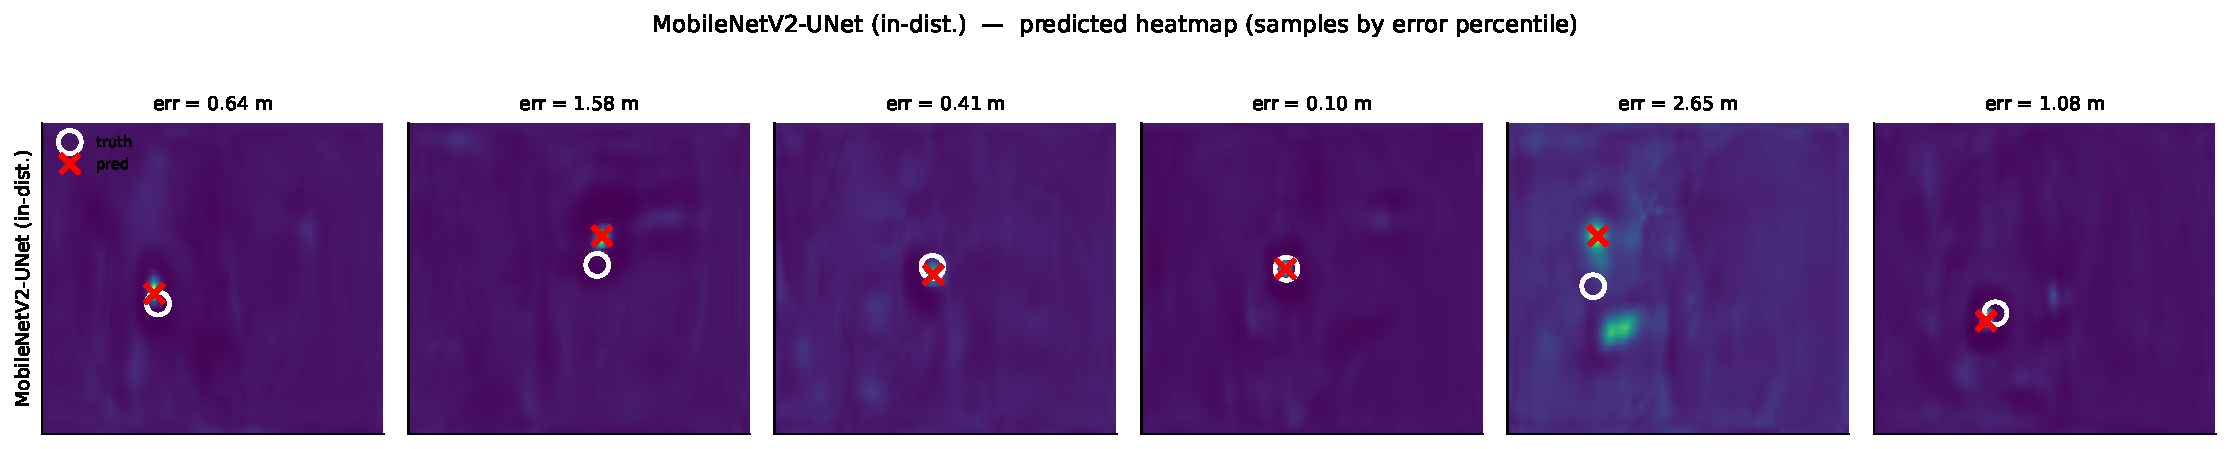
\includegraphics[width=\linewidth]{heatmaps_unet_fig10b.pdf}
\caption{Qualitative in-distribution predictions of the MobileNetV2-UNet. Each panel shows the predicted
heatmap for a test sample drawn at a given error percentile; the white circle marks the ground-truth peak
and the red cross the predicted peak. Low-error cases (left) show tight, single-mode predictions; the
high-error case shows a multimodal heatmap where the chosen peak is displaced.}
\label{fig:res:heatmaps_indist}
\end{figure}

\section{U-Net Architecture and Scheduler Comparison}
\label{sec:res:unet}

We train the MobileNetV2-UNet for 120 epochs with both the cosine-annealing and step-decay learning-rate
schedules, in both its standalone and distilled forms (Table~\ref{tab:res:unet}).

\begin{table}[H]
\centering
\caption{U-Net scheduler and training-mode comparison (120 epochs, $\mathrm{lr}_0 = 10^{-4}$).}
\label{tab:res:unet}
\begin{tabular}{@{}llccc@{}}
\toprule
\textbf{Scheduler} & \textbf{Mode} & \textbf{Median (m)} & \textbf{P90 (m)} & \textbf{P99 (m)} \\
\midrule
Cosine annealing & Standalone & \best{0.640} & 1.523 & 2.750 \\
Step decay       & Standalone & \best{0.640} & 1.552 & 2.918 \\
Cosine annealing & Distilled  & \best{0.640} & \best{1.513} & \best{2.587} \\
\bottomrule
\end{tabular}
\end{table}

The standalone and distilled variants of the MobileNetV2-UNet reach the same median value of 0.640\,m
regardless of the learning-rate schedule. The cosine schedule achieves slightly lower tail percentiles
than the step-decay schedule, with P90 and P99 of 1.523\,m and 2.750\,m for cosine versus 1.552\,m and
2.918\,m for step decay. These results are likely due to the cosine schedule's smooth decay of the
learning rate toward a minimum over the final few epochs of training. For the distilled model, the P99
percentile is further improved to 2.587\,m. The learning-rate schedule therefore has a relatively small
effect on the performance of the model; the architecture is the dominant factor.

\section{Robustness Under Signal Degradation}
\label{sec:res:robustness}

The robustness of each model is evaluated under a variety of signal degradations, with no retraining.
Tables~\ref{tab:res:robust_mobilenet}--\ref{tab:res:robust_unet} report the error of each model under the
full set of corruptions (AP dropout, Gaussian noise, attenuation, and blur), and
Table~\ref{tab:res:noise_summary} summarizes the results under Gaussian noise.

\begin{table}[H]
\centering
\caption{Robustness evaluation --- MobileNetV2 (2.3M). \best{Green bold} = distilled beats standalone.}
\label{tab:res:robust_mobilenet}
\small
\begin{tabular}{@{}lcccc|cccc@{}}
\toprule
 & \multicolumn{4}{c|}{\textbf{Standalone}} & \multicolumn{4}{c}{\textbf{Distilled}} \\
\textbf{Condition} & \textbf{Med.} & \textbf{P90} & \textbf{P99} & \textbf{Mean} & \textbf{Med.} & \textbf{P90} & \textbf{P99} & \textbf{Mean} \\
\midrule
Normal                 & 0.707 & 1.616 & 3.992  & 0.900 & 0.707 & 1.612 & 4.003  & 0.896 \\
Noise $\sigma{=}0.1$   & \worst{16.368}& 20.939& 25.196 & 16.557& \best{4.769} & \best{12.310}& 21.122 & \best{5.953} \\
Noise $\sigma{=}0.2$   & \worst{16.307}& 20.748& 25.188 & 16.503& \best{5.369} & 20.508& 26.014 & \best{7.896} \\
Random 2-AP dropout    & 2.402 & 11.691& 22.997 & 4.468 & 2.516 & 11.631& 21.091 & 4.434 \\
Atten.\ $0.5\times$    & 1.342 & 4.211 & 14.831 & 2.181 & 1.500 & 6.185 & 22.612 & 2.828 \\
Blur $k{=}5$           & 0.849 & 2.121 & 12.033 & 1.281 & 0.854 & 1.924 & 5.839  & 1.125 \\
\bottomrule
\end{tabular}
\end{table}

\begin{table}[H]
\centering
\caption{Robustness evaluation --- TinyCNN (47K). Distillation \emph{harms} dropout robustness.}
\label{tab:res:robust_tinycnn}
\small
\begin{tabular}{@{}lcccc|cccc@{}}
\toprule
 & \multicolumn{4}{c|}{\textbf{Standalone}} & \multicolumn{4}{c}{\textbf{Distilled}} \\
\textbf{Condition} & \textbf{Med.} & \textbf{P90} & \textbf{P99} & \textbf{Mean} & \textbf{Med.} & \textbf{P90} & \textbf{P99} & \textbf{Mean} \\
\midrule
Normal              & 3.922 & 13.919& 23.244 & 5.833 & 3.706 & 14.784& 25.101 & 6.048 \\
Random 1-AP dropout & 7.940 & 16.858& 23.405 & 8.580 & 13.648& 24.502& 28.228 & 12.922\\
Noise $\sigma{=}0.1$& 9.457 & 17.049& 25.018 & 9.946 & 9.439 & 16.568& 23.965 & 9.921 \\
Atten.\ $0.5\times$ & 9.708 & 17.593& 22.233 & 10.318& 18.532& 26.196& 28.343 & 17.829\\
\bottomrule
\end{tabular}
\end{table}

\begin{table}[H]
\centering
\caption{Robustness evaluation --- MobileNetV2-UNet (2.41M). \best{Green bold} = best of the pair.}
\label{tab:res:robust_unet}
\small
\begin{tabular}{@{}lcccc|cccc@{}}
\toprule
 & \multicolumn{4}{c|}{\textbf{Standalone (Cosine)}} & \multicolumn{4}{c}{\textbf{Distilled (Cosine)}} \\
\textbf{Condition} & \textbf{Med.} & \textbf{P90} & \textbf{P99} & \textbf{Mean} & \textbf{Med.} & \textbf{P90} & \textbf{P99} & \textbf{Mean} \\
\midrule
Normal              & 0.640 & 1.581 & 3.651  & 0.851 & 0.640 & 1.513 & 3.587  & 0.829 \\
Noise $\sigma{=}0.1$& \best{3.000}& \best{8.310}& \best{13.873}& \best{3.878}& 3.469 & 10.473& 18.261 & 4.678 \\
Noise $\sigma{=}0.2$& 5.741 & 10.645& 18.137 & 6.050 & \best{5.320} & 12.003& 17.948 & 6.135 \\
Random 2-AP dropout & 3.324 & 13.012& 22.080 & 5.228 & \best{2.730}& \best{8.203}& \best{13.396}& \best{3.711}\\
Blur $k{=}5$        & 0.671 & 1.603 & 3.716  & 0.859 & \best{0.656}& \best{1.526}& 3.943 & \best{0.841} \\
\bottomrule
\end{tabular}
\end{table}

\begin{table}[H]
\centering
\caption{Gaussian-noise robustness summary ($\sigma = 0.1$). \best{Green} = best, \worst{red} = worst.}
\label{tab:res:noise_summary}
\begin{tabular}{@{}llcc@{}}
\toprule
\textbf{Model} & \textbf{Mode} & \textbf{Median (m)} & \textbf{P90 (m)} \\
\midrule
MobileNetV2      & Standalone & \worst{16.368} & \worst{20.939} \\
MobileNetV2      & Distilled  & 4.769  & 12.310 \\
TinyCNN          & Standalone & 9.457  & 17.049 \\
TinyCNN          & Distilled  & 9.439  & 16.568 \\
MobileNetV2-UNet & Standalone & \best{3.000}  & \best{8.310}  \\
MobileNetV2-UNet & Distilled  & 3.469  & 10.473 \\
\bottomrule
\end{tabular}
\end{table}

The MobileNetV2 model with distillation achieves $3.4\times$ greater robustness against Gaussian noise.
The standalone MobileNetV2 model experiences a median error of 16.4\,m when evaluated with $\sigma = 0.1$
Gaussian noise, indicating that it is effectively guessing within the floorplan. The distilled model only
degrades to a median error of 4.8\,m. This is likely due to the fact that during training the model was
trained both against the ground-truth labels and to match the broader predictions of the teacher model,
which regularizes the model's features toward a more noise-robust representation. This is the
spatial-regression analogue of the temperature-scaled soft targets commonly used in classification
distillation~\cite{hinton2015distilling}.

The MobileNetV2-UNet model with skip connections exhibits $5.5\times$ increased robustness against
Gaussian noise. The standalone MobileNetV2-UNet reaches a median error of 3.0\,m, compared to 16.4\,m for
the standalone MobileNetV2. The skip connections provide an additional layer of robustness by allowing
the model to draw on the features learned at the shallow layers of the model, which are less likely to be
corrupted by the noise. The skip connections therefore provide a form of robustness that is independent
of the distillation-based noise robustness.

Interestingly, distilled models with limited fitting capacity exhibit a degradation in performance with
distillation. The distilled TinyCNN model degrades to a median error of 13.6\,m, compared to 7.9\,m for
the standalone model, when evaluated under AP dropout (random 1-AP). This is likely because the limited
capacity of the TinyCNN model causes it to dedicate its capacity to learning the teacher's representation
of the AP interactions; when an AP is removed from the environment at test time, those learned
interactions become invalid, and the model has no remaining capacity to fall back on. There is therefore
a minimum capacity a model must have in order to benefit from knowledge distillation; below roughly
2~million parameters the model degrades in performance with distillation.

These two robustness techniques are not additive in their effects on the MobileNetV2-UNet model. The
standalone model exhibits a median error of 3.0\,m under Gaussian noise, whereas the distilled model
exhibits a median error of 3.47\,m. In this case the architecture-based noise robustness provided by the
skip connections is stronger than the training-based noise robustness introduced through knowledge
distillation.

\section{Cross-Session Generalization}
\label{sec:res:crosssession}

A model that is to be deployed within one or more localizer devices will likely encounter changes in
environment over time, and may need to be deployed in an environment different from the one in which it
was trained. Its generalization to these different environments is therefore of interest. The evaluation
of cross-session generalization is performed in two ways. The first uses the same leave-one-session-out
evaluation used to evaluate the published DLoc model. The second uses a zero-shot evaluation, in which the
models are trained only on the two July sessions yet evaluated on the August sessions.

\subsection{Fair Comparison: Leave-One-Session-Out}
\label{sec:res:crosssession:loso}

We re-ran the MobileNetV2-UNet in the same manner as the published DLoc model, using three random seeds
and leaving out the test session of each fold during training. Table~\ref{tab:res:paper_comparison} and
Figure~\ref{fig:res:crosssession_median} present the results.

\begin{table}[H]
\centering
\caption{Fair comparison with the DLoc paper under the leave-one-session-out protocol (mean $\pm$ std over
3 seeds). Our U-Net uses 2.41M parameters vs.\ DLoc's 16.5M ($6.8\times$ compression). \best{Green bold} =
our result matches or beats the paper.}
\label{tab:res:paper_comparison}
\begin{tabular}{@{}lcccc@{}}
\toprule
\textbf{Held-out session} & \textbf{Median (ours)} & \textbf{Median (paper)} & \textbf{P90 (ours)} & \textbf{P90 (paper)} \\
\midrule
Aug16\_1 (furniture)      & $0.852 \pm 0.044$ & 0.71 & $1.839 \pm 0.067$ & 1.71 \\
Aug16\_3 (diff.\ furn.)   & \best{$0.822 \pm 0.040$} & 0.82 & $2.793 \pm 0.140$ & 2.52 \\
Aug16\_4\_ref (reflector) & $1.116 \pm 0.016$ & 1.05 & \best{$2.489 \pm 0.030$} & 2.77 \\
\midrule
\textbf{Mean}             & \textbf{0.930} & 0.86 & \textbf{2.374} & 2.33 \\
\bottomrule
\end{tabular}
\end{table}

\begin{figure}[H]
\centering
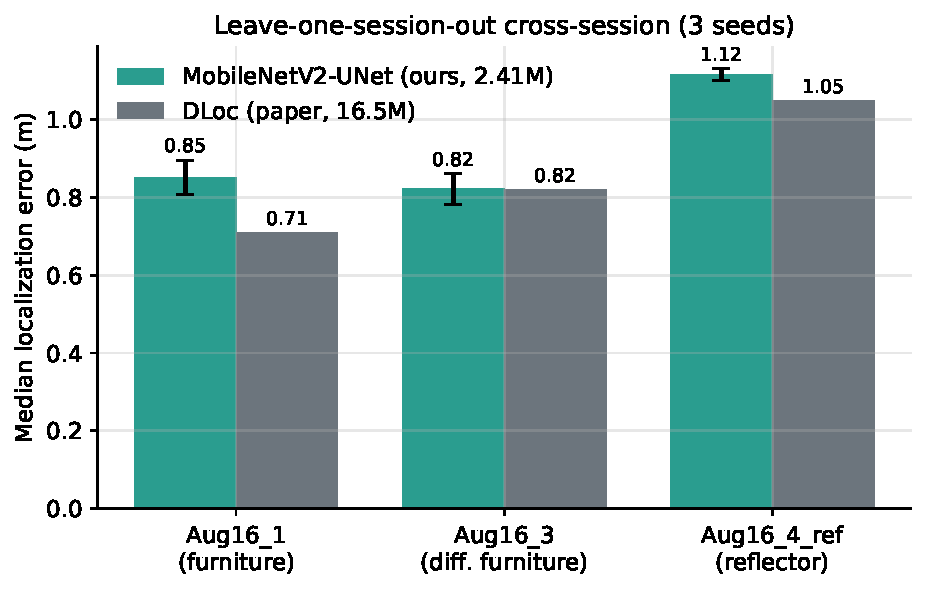
\includegraphics[width=0.74\linewidth]{crosssession_median.pdf}
\caption{Leave-one-session-out median error: our 2.41M-parameter MobileNetV2-UNet (three-seed
mean $\pm$ std) against the published 16.5M-parameter DLoc. The U-Net matches DLoc on the
different-furniture fold and lands within roughly 0.1\,m on the others.}
\label{fig:res:crosssession_median}
\end{figure}

In general, the MobileNetV2-UNet fared similarly to the DLoc model. On the different-furniture fold the
two models are within 0.02\,m of each other (0.822\,m for our model vs.\ 0.82\,m for DLoc); on the
remaining folds the MobileNetV2-UNet's error is within 0.14\,m of DLoc's (averaging 0.930\,m vs.\
0.86\,m). The MobileNetV2-UNet exhibits essentially the same P90 error (2.374\,m vs.\ 2.33\,m on average),
and a \emph{lower} error on the challenging reflector fold (2.489\,m vs.\ 2.77\,m). Such differences are
visible in the heavier tail of the reflector CDF in Figure~\ref{fig:res:cdf_crosssession}. The small
remaining gap on the reflector fold (about 0.07\,m) is expected: the DLoc model includes a consistency
decoder that enforces agreement across the access points, which helps most under the strong specular
multipath introduced by the aluminum reflector, whereas our single-decoder U-Net has no such mechanism.
This is also visible in the qualitative analysis of the predicted heatmaps for the reflector fold
(Figure~\ref{fig:res:heatmaps_cross}). The results are stable across the three random seeds used to train
the model (standard deviations of the median error between 0.016\,m and 0.044\,m), so the MobileNetV2-UNet
reaches similar accuracy to DLoc with $6.8\times$ fewer parameters.

\begin{figure}[H]
\centering
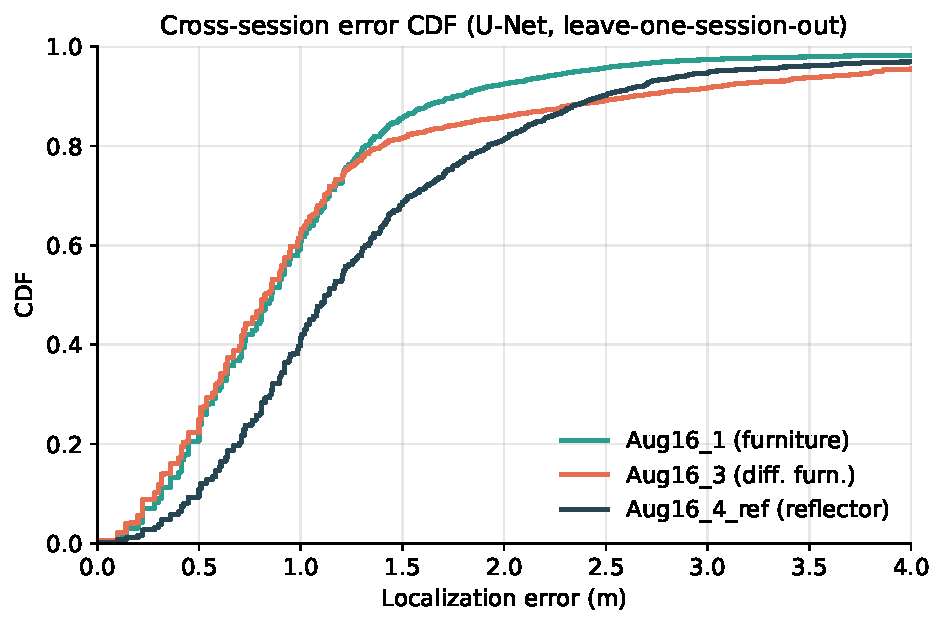
\includegraphics[width=0.78\linewidth]{cdf_crosssession.pdf}
\caption{Cross-session error CDFs for the three held-out folds. The reflector fold (Aug16\_4\_ref) is
clearly the hardest, with its distribution shifted to larger errors, while the two furniture folds track
closely.}
\label{fig:res:cdf_crosssession}
\end{figure}

\begin{figure}[H]
\centering
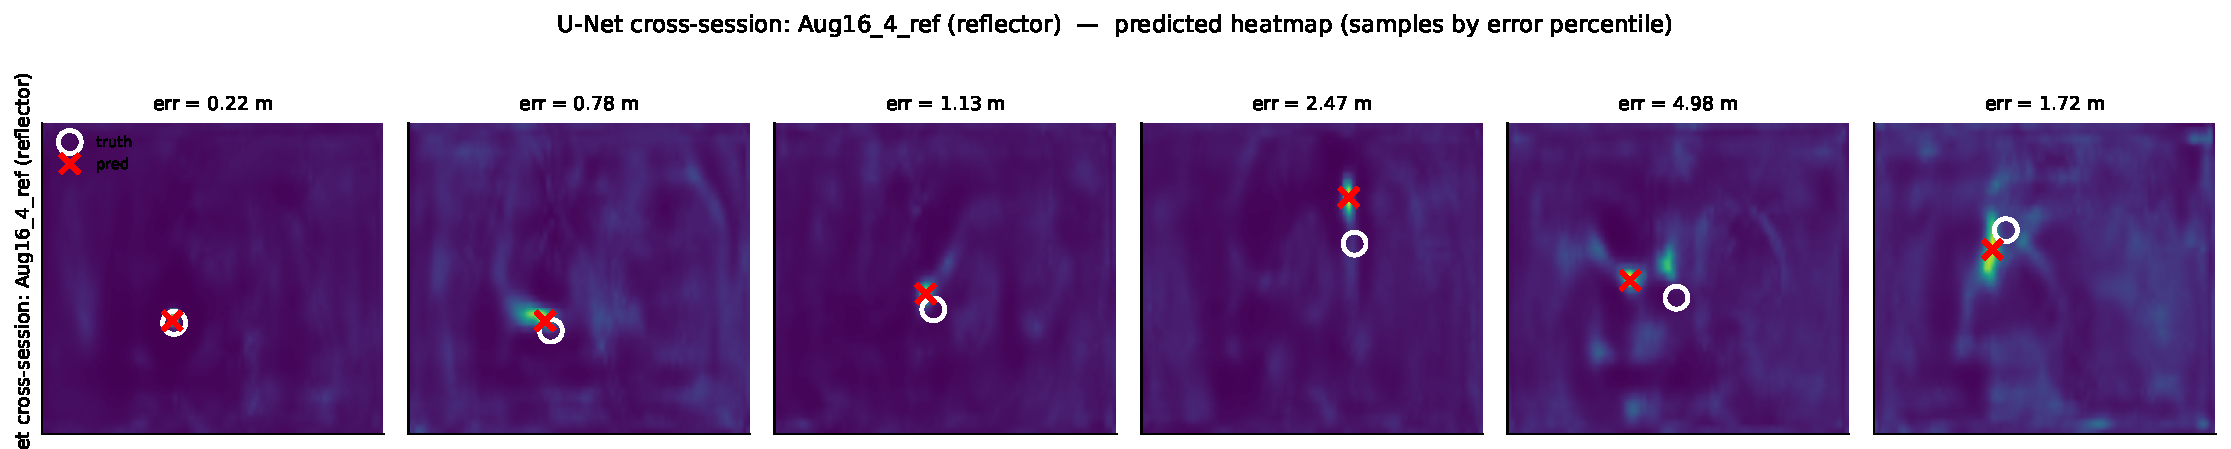
\includegraphics[width=\linewidth]{heatmaps_unet_cross_env4.pdf}
\caption{Qualitative cross-session predictions on the reflector fold (Aug16\_4\_ref). Compared with the
in-distribution panels of Figure~\ref{fig:res:heatmaps_indist}, the heatmaps show additional scattered
probability mass---the specular ``phantom'' reflections introduced by the aluminum panel---which drives
the larger errors on this fold.}
\label{fig:res:heatmaps_cross}
\end{figure}

\subsection{Zero-Shot Stress Test}
\label{sec:res:crosssession:zeroshot}

In addition to the leave-one-session-out evaluation, we evaluated each model in a zero-shot manner,
training each model only on the two July sessions yet evaluating on the August sessions
(Table~\ref{tab:res:zeroshot}). This evaluation is purposely not a fair comparison of each model against
DLoc; it is performed as a means of determining the difference between the architectures and training
techniques.

\begin{table}[H]
\centering
\caption{Zero-shot generalization (2-session training) --- median error (m). An internal
architecture/distillation ablation, \emph{not} a DLoc comparison. \best{Green bold} = best in column.}
\label{tab:res:zeroshot}
\begin{tabular}{@{}llcccc@{}}
\toprule
\textbf{Model} & \textbf{Mode} & \textbf{Sess.~2} & \textbf{Sess.~3} & \textbf{Sess.~4} & \textbf{Sess.~5} \\
\midrule
MobileNetV2   & Standalone & 0.707 & 1.118 & 1.204 & 1.500 \\
MobileNetV2   & Distilled  & 0.707 & 1.118 & 1.204 & 1.442 \\
TinyCNN       & Standalone & 3.922 & 5.964 & 6.327 & 6.605 \\
UNet (Cosine) & Standalone & 0.640 & 1.063 & 1.005 & 1.334 \\
UNet (Cosine) & Distilled  & \best{0.640} & \best{1.020} & \best{1.005} & \best{1.281} \\
\bottomrule
\end{tabular}
\end{table}

Error broadly increases across the August sessions and is highest on the reflector (Session 5) for every model, an indication of the inherent hierarchy in
the difficulty of the sessions, which is a property of the environment rather than of the model. More
interestingly, the benefit of distillation is visible only on the hardest (reflector) fold: it is
negligible for the furniture folds but apparent in the reflector fold for both the MobileNetV2 model
($1.500 \to 1.442$\,m) and the MobileNetV2-UNet model ($1.334 \to 1.281$\,m).

\section{Multi-Seed Statistical Validation}
\label{sec:res:multiseed}

In order to confirm that the differences in performance between the baseline and the student models are
not the result of random initialization, we also trained the baseline model under three different random
seeds (Table~\ref{tab:res:multiseed}).

\begin{table}[H]
\centering
\caption{Multi-seed DLoc baseline (120 epochs, StepLR $\gamma = 0.9$).}
\label{tab:res:multiseed}
\begin{tabular}{@{}lccc@{}}
\toprule
\textbf{Seed} & \textbf{Median (m)} & \textbf{P90 (m)} & \textbf{P99 (m)} \\
\midrule
42  & 0.825 & 2.402 & 22.672 \\
123 & 0.906 & 2.335 &  7.714 \\
777 & 0.894 & 2.102 &  8.694 \\
\midrule
\textbf{Mean $\pm$ Std} & $\mathbf{0.875 \pm 0.036}$ & $\mathbf{2.280 \pm 0.128}$ & $\mathbf{13.027 \pm 6.832}$ \\
\bottomrule
\end{tabular}
\end{table}

These multi-seed runs use the full 120-epoch schedule and reach a mean median of 0.875\,m, above the
0.707\,m of the 50-epoch run reported in Table~\ref{tab:res:baseline}: because the StepLR schedule
($\gamma = 0.9$) never decays the learning rate to zero, longer training drifts slightly upward. The
median varied by only $\pm 0.036$\,m across the three seeds (coefficient of variation 4.1\%), indicating
that the baseline accuracy is stable across random initializations. P99, however, varied by $\pm 6.832$\,m (CV 52\%), because the P99
calculation depends on a small number of inherently ambiguous locations whose accuracy varied between
seeds. Furthermore, the U-Net's median accuracy of 0.640\,m is 6.5 standard deviations away from the mean
accuracy of the baseline (0.875\,m), indicating the significance of the accuracy improvement that results
from the architectural change from DLoc to the U-Net.

\section{Computational Efficiency}
\label{sec:res:efficiency}

The deployment cost of each model is reported in Table~\ref{tab:res:efficiency}: the number of parameters
of each model, the number of floating-point operations required to run the model (with dummy inputs at a
batch size of one), and the inference latency of the model on both CPU and GPU platforms. Figures
\ref{fig:res:pareto} and~\ref{fig:res:params} show the accuracy of the models in relation to model size
and the parameter count of each model.

\begin{table}[H]
\centering
\caption{Computational efficiency (batch size 1). FLOPs and latency measured with the built-in PyTorch
flop counter and timed runs. The DLoc figure is its test-time encoder+decoder.}
\label{tab:res:efficiency}
\begin{tabular}{@{}lrrrr@{}}
\toprule
\textbf{Model} & \textbf{Params} & \textbf{FLOPs} & \textbf{CPU (ms)} & \textbf{GPU (ms)} \\
\midrule
DLoc baseline    & 16.5M  & 81.06G & 270.9 & 16.2 \\
MobileNetV2      & 2.27M  & 1.28G  & 17.9  & 6.3  \\
TinyCNN          & 47K    & 0.66G  & 9.1   & 1.5  \\
MobileNetV2-UNet & 2.41M  & \best{1.45G} & \best{27.2} & \best{4.5} \\
\bottomrule
\end{tabular}
\end{table}

\begin{figure}[H]
\centering
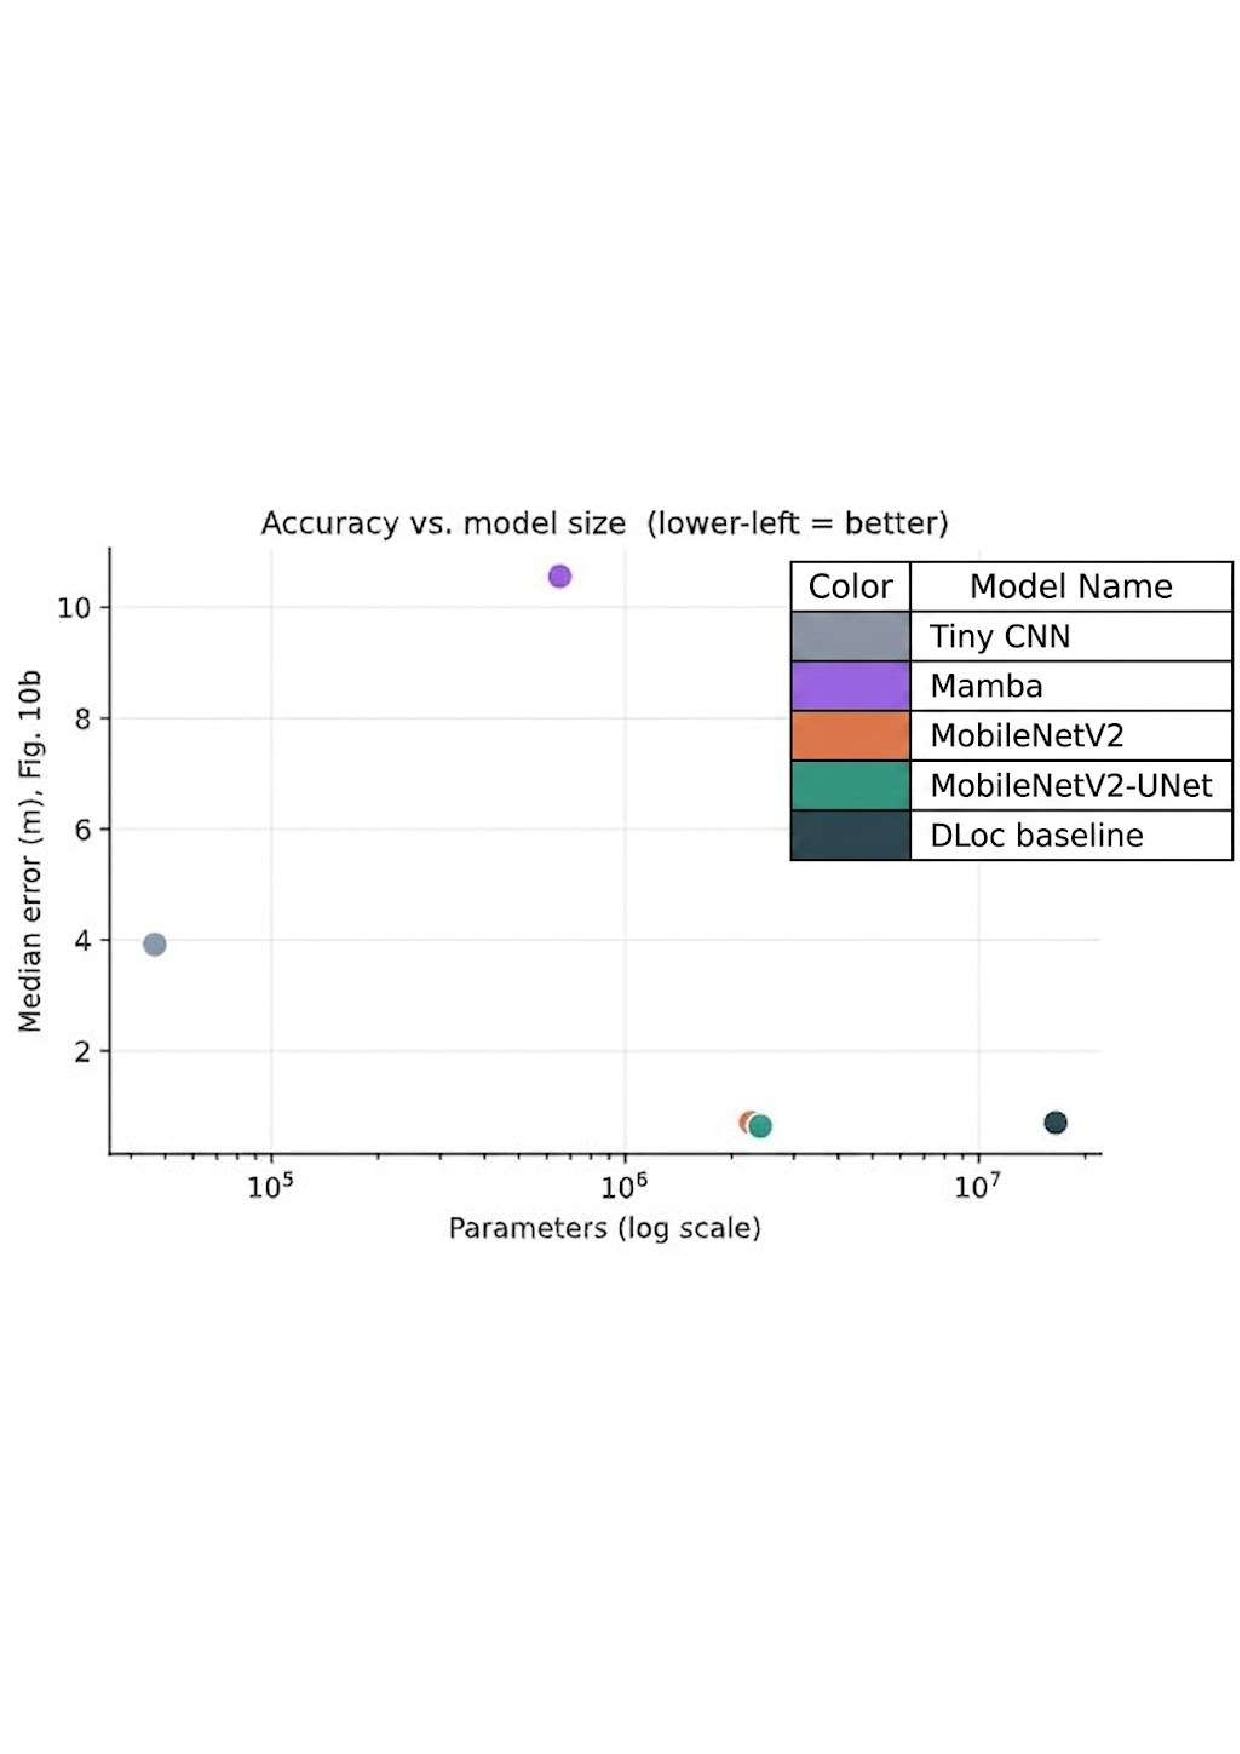
\includegraphics[width=0.7\linewidth]{compression_pareto.pdf}
\caption{Accuracy versus model size. The MobileNetV2-UNet sits at the favorable lower-left of the
accuracy--size plane, achieving the best median error among all models at a fraction of the DLoc parameter
count.}
\label{fig:res:pareto}
\end{figure}

\begin{figure}[H]
\centering
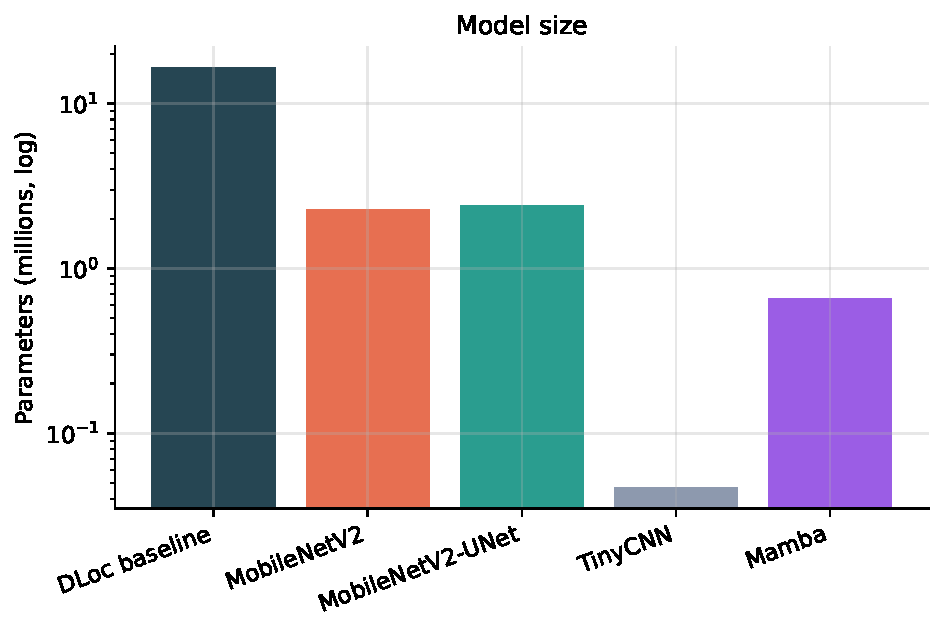
\includegraphics[width=0.7\linewidth]{compression_params.pdf}
\caption{Parameter counts of each model (log scale).}
\label{fig:res:params}
\end{figure}

The MobileNetV2-UNet model achieves an accuracy of 0.640\,m with only 1.45\,GFLOPs and 27.2\,ms of CPU
inference latency, compared to the DLoc baseline's 81.06\,GFLOPs and 270.9\,ms. The MobileNetV2-UNet thus
reduces computational cost by a factor of 56 and improves CPU inference time by a factor of 10---on the
platform most representative of edge deployment. The U-Net model is also $3.6\times$ faster than DLoc on
the GPU. The accuracy improvement achieved by the MobileNetV2-UNet is therefore not gained at the expense
of increased computational cost relative to the DLoc teacher.

\section{Discussion}
\label{sec:res:discussion}

\paragraph{The dual nature of knowledge distillation.} Knowledge distillation in this task differs from
its use in models such as classifiers. In the spatial-localization task, the teacher's outputs are
inherently uncertain about the specific location and instead provide a heatmap of possible locations.
The resulting smoothing provides no benefit in the in-distribution case, but is beneficial under noise
and in generalization to cross-session folds, while being harmful to the smallest model (TinyCNN). The
knowledge-distillation signal therefore has two seemingly opposite effects on student models of different
capacities.

\paragraph{Two complementary robustness mechanisms.} The two robustness mechanisms provided by the
MobileNetV2-UNet model are complementary rather than additive. One might therefore expect diminishing, or
even negative, returns from combining the architectural robustness of the skip connections with the
training-based robustness of knowledge distillation. An understanding of which type of corruption to
expect is required in order to choose which mechanism will be most beneficial: the skip connections
protect against high-noise environments, and knowledge distillation against the failure of multiple
access points.

\paragraph{Practical recommendation.} In general, the distilled MobileNetV2-UNet outperforms the other
models in each category: it achieves an in-distribution accuracy of 0.640\,m, attains competitive
cross-session accuracy while being $6.8\times$ smaller than DLoc, exhibits the best results under multi-AP
dropout, and incurs $56\times$ lower computational cost than the DLoc model. If noise robustness is the
main concern, the standalone U-Net may be preferred; if model compression is the main concern, the
distilled plain MobileNetV2 achieves an accuracy of 0.707\,m with only 2.3M parameters. In each case, a
model roughly an order of magnitude smaller than DLoc achieves the same accuracy---the main point of this
thesis.
